\documentclass[oneside, final, 12pt]{article}

\pagestyle{plain}

\usepackage{a4wide}
\usepackage[utf8]{inputenc}
\usepackage[russian]{babel}
\usepackage{vmargin}
\setpapersize{A4}
\setmarginsrb{2cm}{1.5cm}{1cm}{1.5cm}{5pt}{5mm}{5pt}{13mm}
\usepackage{indentfirst}
\usepackage{graphicx}

\usepackage{amsmath}
\usepackage{amsfonts}
\usepackage{amsthm}
\usepackage{amssymb}

\def\hevKul{\chi(t)}
\def\lftKul{\supset}
\def\bsbKul{\boldsymbol }

\newtheoremstyle{def}
        {\topsep}
        {\topsep}
        {\normalfont}
        {\parindent}
        {\bfseries}
        {.}
        {.5em}
        {}
\theoremstyle{def}
\newtheorem{definition}{Определение}[section]
\newtheorem{example}{Пример}[section]

\begin{document}

\thispagestyle{empty}

\begin{center}
\ \vspace{-3cm}


\includegraphics[width=0.5\textwidth]{pict/msu.pdf}\\
{\scshape Московский государственный университет имени М.~В.~Ломоносова}\\
Факультет вычислительной математики и кибернетики\\
Кафедра системного анализа

\vfill

\vspace{5cm}

{\Huge\bfseries <<ПЛФ: лекция 10>>}
\end{center}

\vspace{3cm}

\begin{flushright}
    \large
    \textit{Студент 415 группы}\\
    И.~А.~Кулешов
    \vspace{5mm}
    
    \textit{Руководитель практикума}\\
    к.ф.-м.н, доцент П.~А.~Точилин
\end{flushright}

\vfill

\begin{center}
Москва, 2019
\end{center}

\newpage

	\begin{center}
	\section{Преобразования Лапласа}
	\end{center}
	\subsection{Введение}
	\begin{minipage}{0.4\textwidth}
		Будем рассматривать $f_{\mu}(t):$
		$$
	  		f_{\mu}(t)=f(t)e^{-\mu t}, 
		 $$
		где $f(t) = 0 \text{ при }  t<0$. \newline
		
		Функция Хевисайда: 
		$$\chi (t) = 	\begin{cases}
							1, & t \geqslant 0,\\	
							0, & t < 0.
						\end{cases}$$	
		
		
		Если домножить $f(t)$ на $\chi(t)$ выйдет: 
		$$
		  f(t)\chi(t) =
		  	\begin{cases}
		  		f(t), & t \geqslant 0 ,\\
		  		0, & t<0.
		  	\end{cases} 
		$$
	\end{minipage}
	\hfill
	\begin{minipage}{0.6\textwidth}
		\centering Пример: 
		
		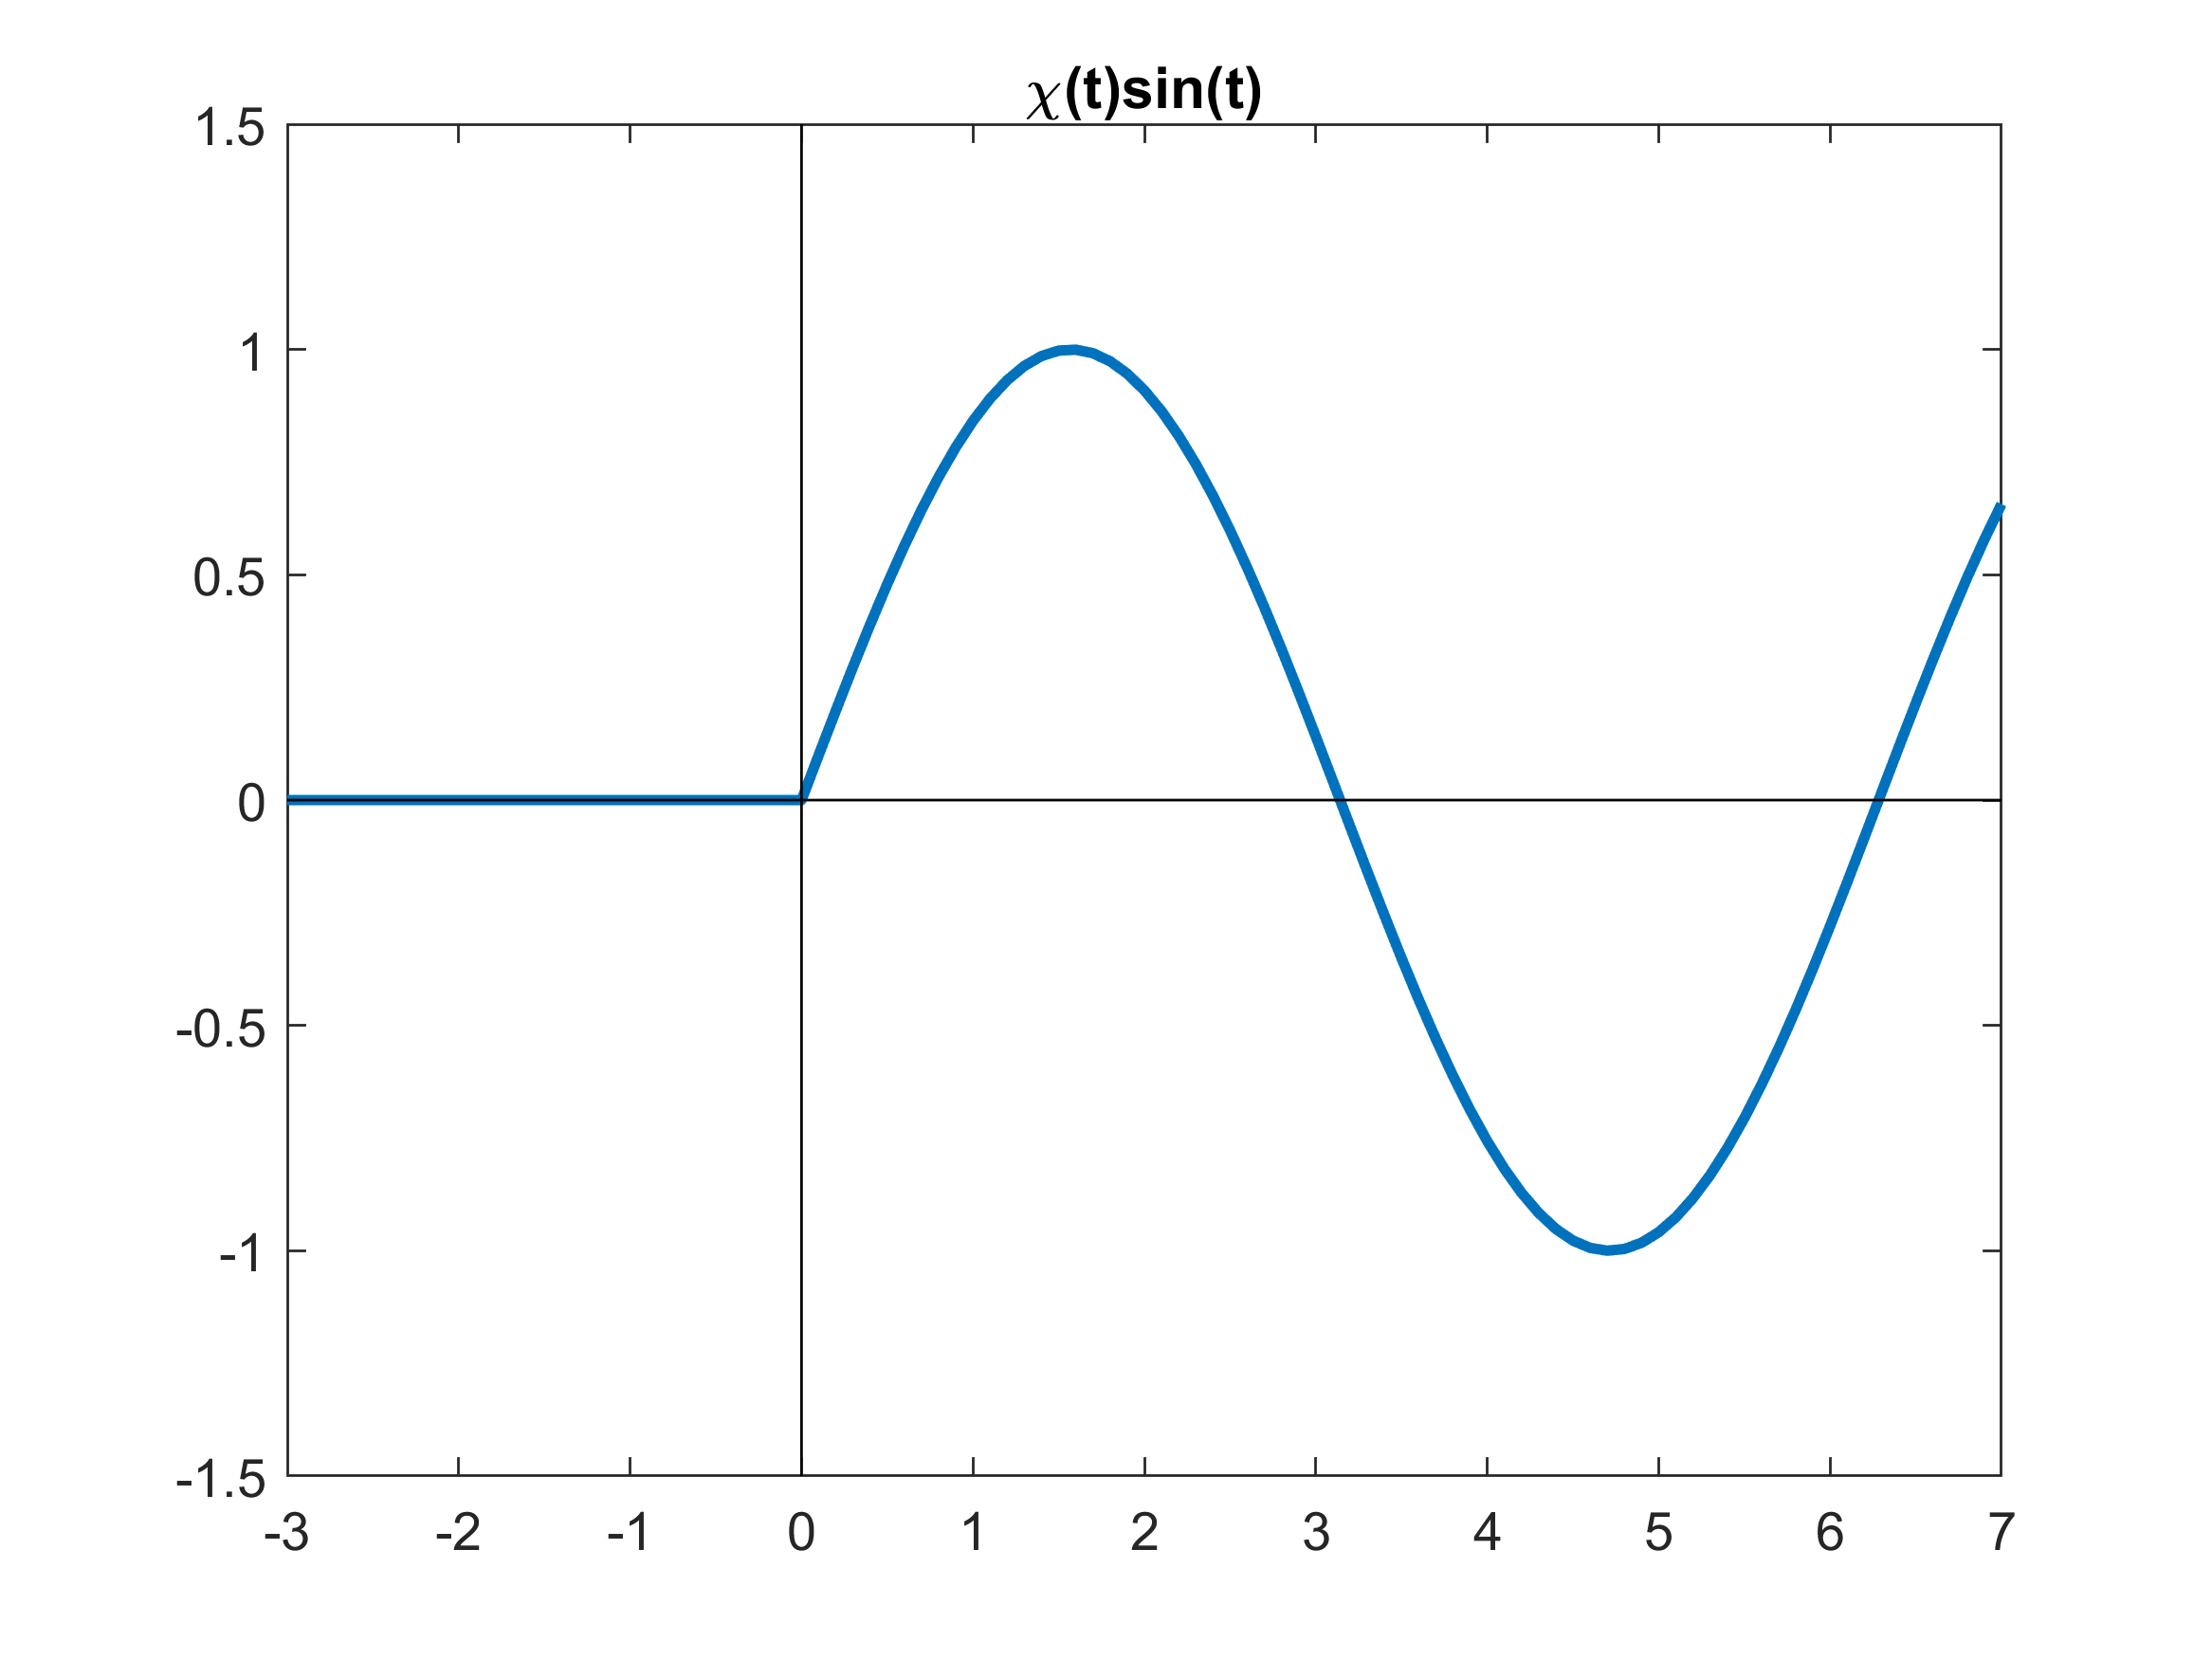
\includegraphics[width=0.9\textwidth]{pict/hev_pict.png}
	\end{minipage} \newline
	
	$$
	\begin{gathered}
		\large F_{\mu}(\lambda) 	= \int\limits_{-\infty}^{+\infty}f_{\mu}(t)e^{-i\lambda t} dt 
											 	= \int\limits_{0}^{+\infty}f(t)e^{-(\mu+i\lambda) t} dt =
											 	\{ \underline{p = \mu +i\lambda}\} =
											 	 \int\limits_{0}^{+\infty}f(t)e^{-p t} dt = 
											 	 F(p), \qquad p \in \mathbb{C}. \\							 	
	 	f(t)e^{-\mu t} = \dfrac{1}{2\pi} \int\limits_{-\infty}^{+\infty} F(\mu+i\lambda)e^{i\lambda t} d \lambda
	 		 \Rightarrow 
	 		 	f(t) =  \dfrac{1}{2\pi} \int\limits_{-\infty}^{+\infty} F(\mu+i\lambda)e^{(\mu +i\lambda) t} d \lambda
	 		 		=   \dfrac{1}{2\pi i} \int\limits_{\mu-i\infty}^{\mu+i\infty} F(p)e^{pt} d t. \\
	 \end{gathered}
	$$
	
	\begin{minipage}{0.4\textwidth}
		$
			\begin{gathered}
			 	\textbf{Преобразование Лапласа:} \qquad
			 		F(p) = \int\limits_{0}^{+\infty} f(t) e^{-pt}dt,  \\
				\textbf{Формула Меллина:} \qquad	
					f(t) =  \dfrac{1}{2\pi i} \int\limits_{\mu-i\infty}^{\mu+i\infty} F(p)e^{pt} d t. 
			\end{gathered} 
		$
	\end{minipage}
	\hfill
	\begin{minipage}{0.3\textwidth}
		\textbf{Преобразование \\ несимметрично!} \vspace{3mm}
	\end{minipage} \newline
	\noindent
	При $\textrm{Re}\, p >\widetilde{\mu}$ мы не выйдем из класса приемлемых функций: $F(p)$ -- определена.
	
	Пусть $M_f = \left\{ \mu \in \mathbb{R}: \exists \int\limits_{0}^{+\infty}|f(t)e^{-\mu t}|dt \right \}$. 
	Если $\mu_1\in M_f$, то $\forall \mu_2\geqslant \mu_1 \Rightarrow \mu_2 \in M_f$. \newline
	Рассматриваются $f: M_f \neq \varnothing$. Абсцисса сходимости $\boldsymbol{\widetilde{\mu}} 
		\boldsymbol{= }\inf\{ \mu \in M_f\} \in [-\infty,+\infty].$ \newline
	Продифференцируем $F(p)=\int\limits_{0}^{+\infty}f(t) e^{-pt}dt$ по $p$ и для $\forall\mu>\widetilde{\mu}$:
	$$
		\begin{gathered}
			\int\limits_{0}^{+\infty} \left|(-t)f(t) e^{-pt}\right|dt  = 
						\begin{Bmatrix}	
							\mu - \widetilde{\mu} = \Delta \mu >0, \\
							\mu = \frac{\Delta \mu}{2} + \mu - \frac{\Delta \mu}{2}, \\
							\text{причем } \mu - \frac{\Delta \mu}{2} > \widetilde{\mu}
						\end{Bmatrix} 
						= \int\limits_{0}^{+\infty}  \left|(-t) f(t) e^{-\frac{\Delta \mu}{2} t}
																			e^{-\left(\mu - \frac{\Delta \mu}{2}\right)t}
																			e^{-i\lambda t} \right| dt = \\
						= \int\limits_{0}^{+\infty}  \left|(-t)e^{-\frac{\Delta \mu}{2} t} \right|
																   \left|  f(t) e^{-\left(\mu - \frac{\Delta \mu}{2}\right)t} \right|
																 	\left|	e^{-i\lambda t} \right| dt =
												\begin{Bmatrix}	
													\left|(-t)e^{-\frac{\Delta \mu}{2} t} \right| \text{ -огранич.}\\
													\left|  f(t) e^{-\left(\mu - \frac{\Delta \mu}{2}\right)t} \right| \in M_f \\
													\left|	e^{-i\lambda t} \right| = 1
												\end{Bmatrix} \Rightarrow F'(p) \in M_f.
		\end{gathered}	
	$$
	 
	Получаем:
	$$
		\begin{gathered}
			F'(p) = \int\limits_{0}^{+\infty} (-t)f(t) e^{-pt}dt, \\
			F^{(k)}(p)=  \int\limits_{0}^{+\infty} (-t)^{(k)}f(t) e^{-pt}dt. 
		\end{gathered}\qquad \textrm{Re}\, p > \widetilde\mu \quad \Rightarrow \quad
					 F(p) - \text{ аналитическая при }\textrm{Re}\, p > \widetilde\mu
	$$
		
		Часть $F$ является мероморфной, т.е. аналитической за исключением конечного числа особых точек,
		которые являются полюсами или устранимыми особыми точками. \newline
	
	\begin{minipage}{0.5\textwidth}	
	
		\centering{Перевернутая лемма Жордана} \newline
		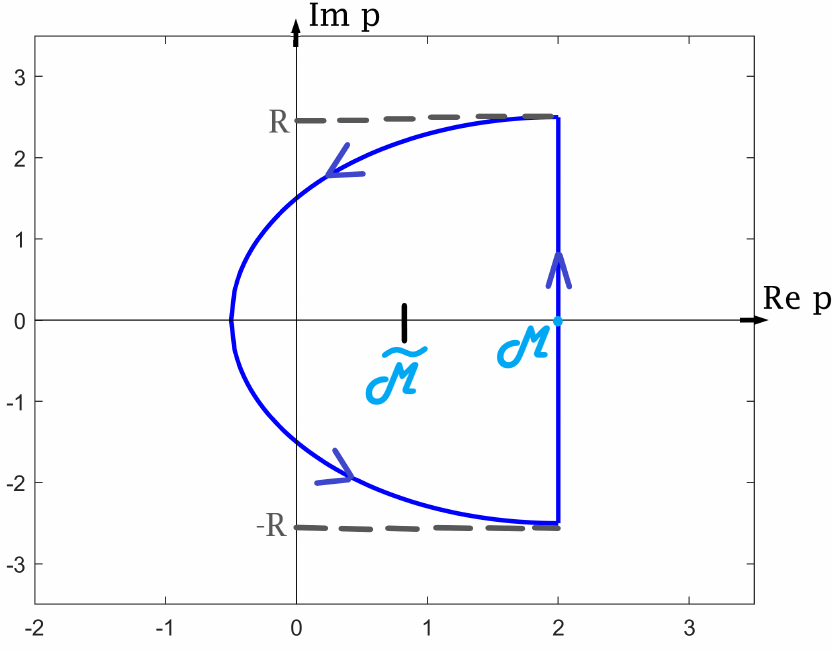
\includegraphics[width=0.85\textwidth]{pict/analit_pict.png}
	\end{minipage}
	\hfill
	\begin{minipage}{0.4\textwidth}
		$
		\begin{gathered}
	 		f(t) =\dfrac{1}{2\pi i} 2\pi i \sum\limits_{p=p_j}\textrm{Res} [F(p)e^{pt}] \Rightarrow \\
	 		\underline{\textbf{\large!} \quad f(t) = \sum\limits_{p=p_j}\textrm{Res} [F(p)e^{pt}] \quad \textbf{\large!}}
		\end{gathered} \vspace{10mm}
		$
		\newline
		$\exists A \geqslant 0 \, \mu_0 \in \mathbb{R} \, |f(t)|\leqslant Ae^{\mu_0 t}\Rightarrow 
			\widetilde\mu \leqslant \mu_0$
	\end{minipage} \newline
	
	\begin{center}
		Будем обозначать соответствие следующим образом: 
			$\mathbf{f(t) \supset F(p)}: \quad 
				\begin{gathered}
					\mathbf{f(t)} \text{ --- оригинал} \\
					\mathbf{F(p)} \text{ --- изображение} 
				\end{gathered}
			$
	\end{center}
		
	 \begin{center}\subsection{Таблица преобразований:}\end{center}
	Простые:
	\begin{itemize}
		\item $\chi(t) \lftKul \dfrac{1}{p}$
		\item 	
				\begin{minipage}{0.4\textwidth}
					$$
					\begin{cases}
						\hevKul t^{\alpha} \lftKul \dfrac{\Gamma(\alpha+1)}{p^{\alpha+1}},\,\, \alpha > -1 \vspace{3mm}\\
						\hevKul t^{n} \lftKul \dfrac{n!}{p^{n+1}}\,\,
					\end{cases} 
					$$
				\end{minipage}
					\hfill
				\begin{minipage}{0.5\textwidth}
						$$
						\begin{gathered}
							\int\limits^{\infty}_{0} t^{\alpha}e^{-pt} = 
					 							\begin{Bmatrix}	
													p>0, p\in \mathbb{R}, \\
													 pt = s\\
												\end{Bmatrix} = 
												\int\limits^{\infty}_{0} \dfrac{s^{\alpha}}{p^{\alpha}}e^{-s}\dfrac{ds}{p} =\\
												=\dfrac{1}{p^{\alpha}} \int\limits^{\infty}_{0} s^{\alpha} e^{-s} ds 
												= \dfrac{\Gamma(\alpha+1)}{p^{\alpha}}
						\end{gathered}
						$$
				\end{minipage}
		\item 
				\begin{minipage}{0.4\textwidth}
					$
					\begin{cases}
						\hevKul t^{\alpha}e^{\beta t} \lftKul 
									\dfrac{\Gamma(\alpha+1)}{(p-\beta)^{\alpha+1}} \vspace{3mm}\\
						\hevKul t^{n}e^{\beta t} \lftKul \dfrac{n!}{(p-\beta)^{n+1}}\,\
					\end{cases} 
					$
				\end{minipage}
					\hfill
				\begin{minipage}{0.5\textwidth}
					 $\left[ \quad \begin{gathered}
					 				\\
					 				\text{от $t^\alpha$ появляется $\Gamma(\alpha+1)$ и везде $p^{\alpha+1}$} \\
					 				\text{от $e^{\beta t}$ появляется $(p-\beta)$}
					 				\\ \,
					 			\end{gathered} \quad
					 	\right]$
				\end{minipage}				 	
	\end{itemize}
	\vspace{20mm}	
	Тригонометрические:
	\begin{itemize}
		\item $\mathbf{cos(}$$\bsbKul w$$\bsbKul t)$ \newline
			\begin{minipage}{0.5\textwidth}
			$
				\begin{cases}
					\hevKul t^{\alpha} \cos(\omega t) \lftKul 
							\dfrac{\Gamma(\alpha+1)}{2}\left[ \dfrac{1}{(p+i\omega)^{\alpha+1}}
									\stackrel{\bsbKul!}{\bsbKul+}
										\dfrac{1}{(p-i\omega)^{\alpha+1}}
										\right] \vspace{4mm} \\
					\begin{gathered}
						\hevKul \cos(\omega t)  \lftKul 
									\dfrac{p}{p^2+\omega^2}, \vspace{4mm}\\
						\hevKul e^{\beta t}\cos(\omega t) \lftKul \dfrac{(p-\beta)}{(p-\beta)^2+\omega^2},\,\,
					\end{gathered} \qquad \text{ $\bsbKul p$ сверху}
				\end{cases} 
			$	
			\end{minipage}
					\hfill
			\begin{minipage}{0.5\textwidth}
				$$
				\left| \quad
					\begin{gathered}
					\quad\cos(\omega t) = \dfrac{e^{i\omega t}+e^{-i\omega t}}{2} \Rightarrow \quad \\
					\begin{gathered}
						\hevKul t^{\alpha}e^{i\omega t}  \lftKul \dfrac{\Gamma(\alpha+1)}{(p-i\omega)^{\alpha+1}},
								 \vspace{3mm}\\+ \\
						\hevKul t^{\alpha}e^{-i\omega t} \lftKul \dfrac{\Gamma(\alpha+1)}{(p+i\omega)^{\alpha+1}},\,\,
					\end{gathered}\quad  \vspace{3mm}
					\end{gathered} \right.
				$$
			\end{minipage}
			\item $\mathbf{sin(}$$\bsbKul w$$\bsbKul t)$ \newline
				$
					\begin{cases}
						\hevKul t^{\alpha} \sin(\omega t) \lftKul 
								\dfrac{\Gamma(\alpha+1)}{2}\left[ \dfrac{1}{(p+i\omega)^{\alpha+1}}
										\stackrel{\bsbKul!}{\bsbKul-}
											\dfrac{1}{(p-i\omega)^{\alpha+1}}
											\right] \vspace{4mm} \\
						\begin{gathered}
							\hevKul \sin(\omega t)  \lftKul 
										\dfrac{\omega}{p^2+\omega^2}, \vspace{4mm}\\
							\hevKul e^{\beta t}\sin(\omega t) \lftKul \dfrac{\omega}{(p-\beta)^2+\omega^2},\,\,
						\end{gathered}  \qquad \text{ $\bsbKul w$ сверху}
					\end{cases} \vspace{4mm}
				$	
	\end{itemize}
	Гиперболические:
	\begin{itemize}
		\item $\mathbf{cosh(}$$\bsbKul w$$\bsbKul t)$ \newline
			\begin{minipage}{0.5\textwidth}
			$ \left.
				\begin{cases}
						\hevKul \cos(\omega t)  \lftKul 
									\dfrac{p}{p^2-\omega^2}, \vspace{4mm}\\
						\hevKul e^{\beta t}\cos(\omega t) \lftKul \dfrac{(p-\beta)}{(p-\beta)^2-\omega^2},\,\,
				\end{cases} \text{ <<$\bsbKul-$>> в знаменателе}  \quad  \right| 
			$	
			\end{minipage}
					\hfill
			\begin{minipage}{0.5\textwidth}
				$$
					\qquad \, \quad  \cosh(\omega t) = \dfrac{e^{-\omega t}+e^{\omega t}}{2}
				$$
			\end{minipage}
			\item $\mathbf{sin(}$$\bsbKul w$$\bsbKul t)$ \newline
				$
					\begin{cases}
						\begin{gathered}
							\hevKul \sin(\omega t)  \lftKul 
										\dfrac{\omega}{p^2+\omega^2}, \vspace{4mm}\\
							\hevKul e^{\beta t}\sin(\omega t) \lftKul \dfrac{\omega}{(p-\beta)^2-\omega^2},\,\,
						\end{gathered} \quad \text{ <<$\bsbKul-$>> в знаменателе}
					\end{cases} \vspace{10mm}
				$	
	\end{itemize}

	\noindent	
	Рассмотрим формулу Меллина: $f(t) = \sum\limits_{p=p_j}\textrm{Res} [F(p)e^{pt}] $
	
	\begin{minipage}{0.6\textwidth}	
		$$
			\begin{gathered}
				F(p)e^{pt} \stackrel{R \rightarrow \infty}{\Rightarrow} 0 \\
				p = \mu + \textrm{Re } e^{i\varphi t}
			\end{gathered} \quad \text{ равномерно по } \varphi \in \left[\frac{\pi}{2}; \frac{3\pi}{2}\right]
		$$
	\end{minipage}
	\hfill
	\begin{minipage}{0.4\textwidth}	
		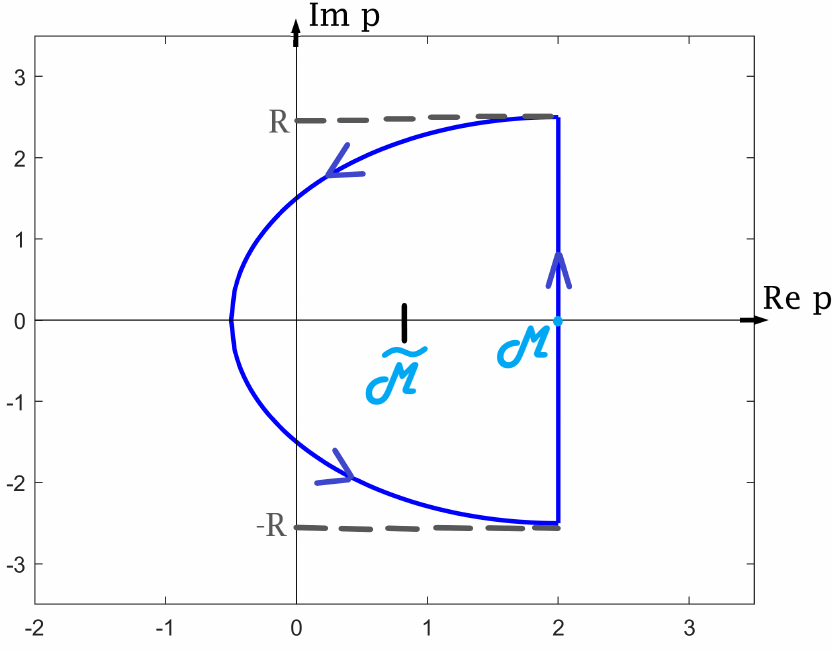
\includegraphics[width=0.85\textwidth]{pict/analit_pict.png}
	\end{minipage} \newline
	\noindent
	\begin{example}
	$$		
			F(p) = \dfrac{1}{(p+1)(p+2)} \qquad f(t) = ? \vspace{2mm}
	$$
	$
		\begin{gathered}
			F(p)e^{pt} = \dfrac{c_{-1}}{p+1} +c_0 + c_1(p+1) + \cdots  \vspace{3mm} \\
			\left| \begin{gathered}
						p_1 = -1: \quad \lim_{p\to-1}\dfrac{(p+1)e^{pt}}{(p+1)(p+2)} \rightarrow e^{-t} \\
						p_2 = -2: \quad \lim_{p\to-2}\dfrac{(p+2)e^{pt}}{(p+1)(p+2)} \rightarrow -e^{-2t}
					\end{gathered} \right. \qquad \Rightarrow \quad
						f(t) = e^{-t} -  e^{-2t} \vspace{2mm}\\			
		\end{gathered}  
	$\newline
	\end{example}
	\subsection{Свойства преобразования Лапласа}
	\renewcommand{\labelenumi}{\fbox{ \large\Roman{enumi} }}
	\renewcommand{\labelenumii}{\arabic{enumii}.}
	\begin{enumerate}
		\item \textbf{Линейные подстановки}
			 \begin{enumerate}
			 	\item Th подобия \vspace{4mm} \newline
			 		\begin{minipage}{0.4\textwidth}	
			 			$
			 				\begin{gathered}
		 						f(at) \lftKul \dfrac{1}{a}F\left(\dfrac{p}{a}\right),\,  a>0  \qquad \vspace{3mm} \left| 
		 						 \qquad \int\limits_{0}^{+\infty} f(at) e^{-pt}dt  \quad \{s=at\}
		 						\vspace{3mm}\right.
		 					\end{gathered}
						$
						$
							\dfrac{1}{b} f\left(\dfrac{t}{b}\right) \lftKul F(pb), \quad b = \dfrac{1}{a}> 0
						$
			 		\end{minipage} \vspace{5mm}
			 	\item 1-ая Th смещения \vspace{1mm} \newline
			 		$$
			 			\chi(t-a)f(t-a)  \lftKul e^{-ap}F(p),\,  a>0
			 		$$
			 		
			 		\begin{minipage}{0.45\textwidth}	
			 			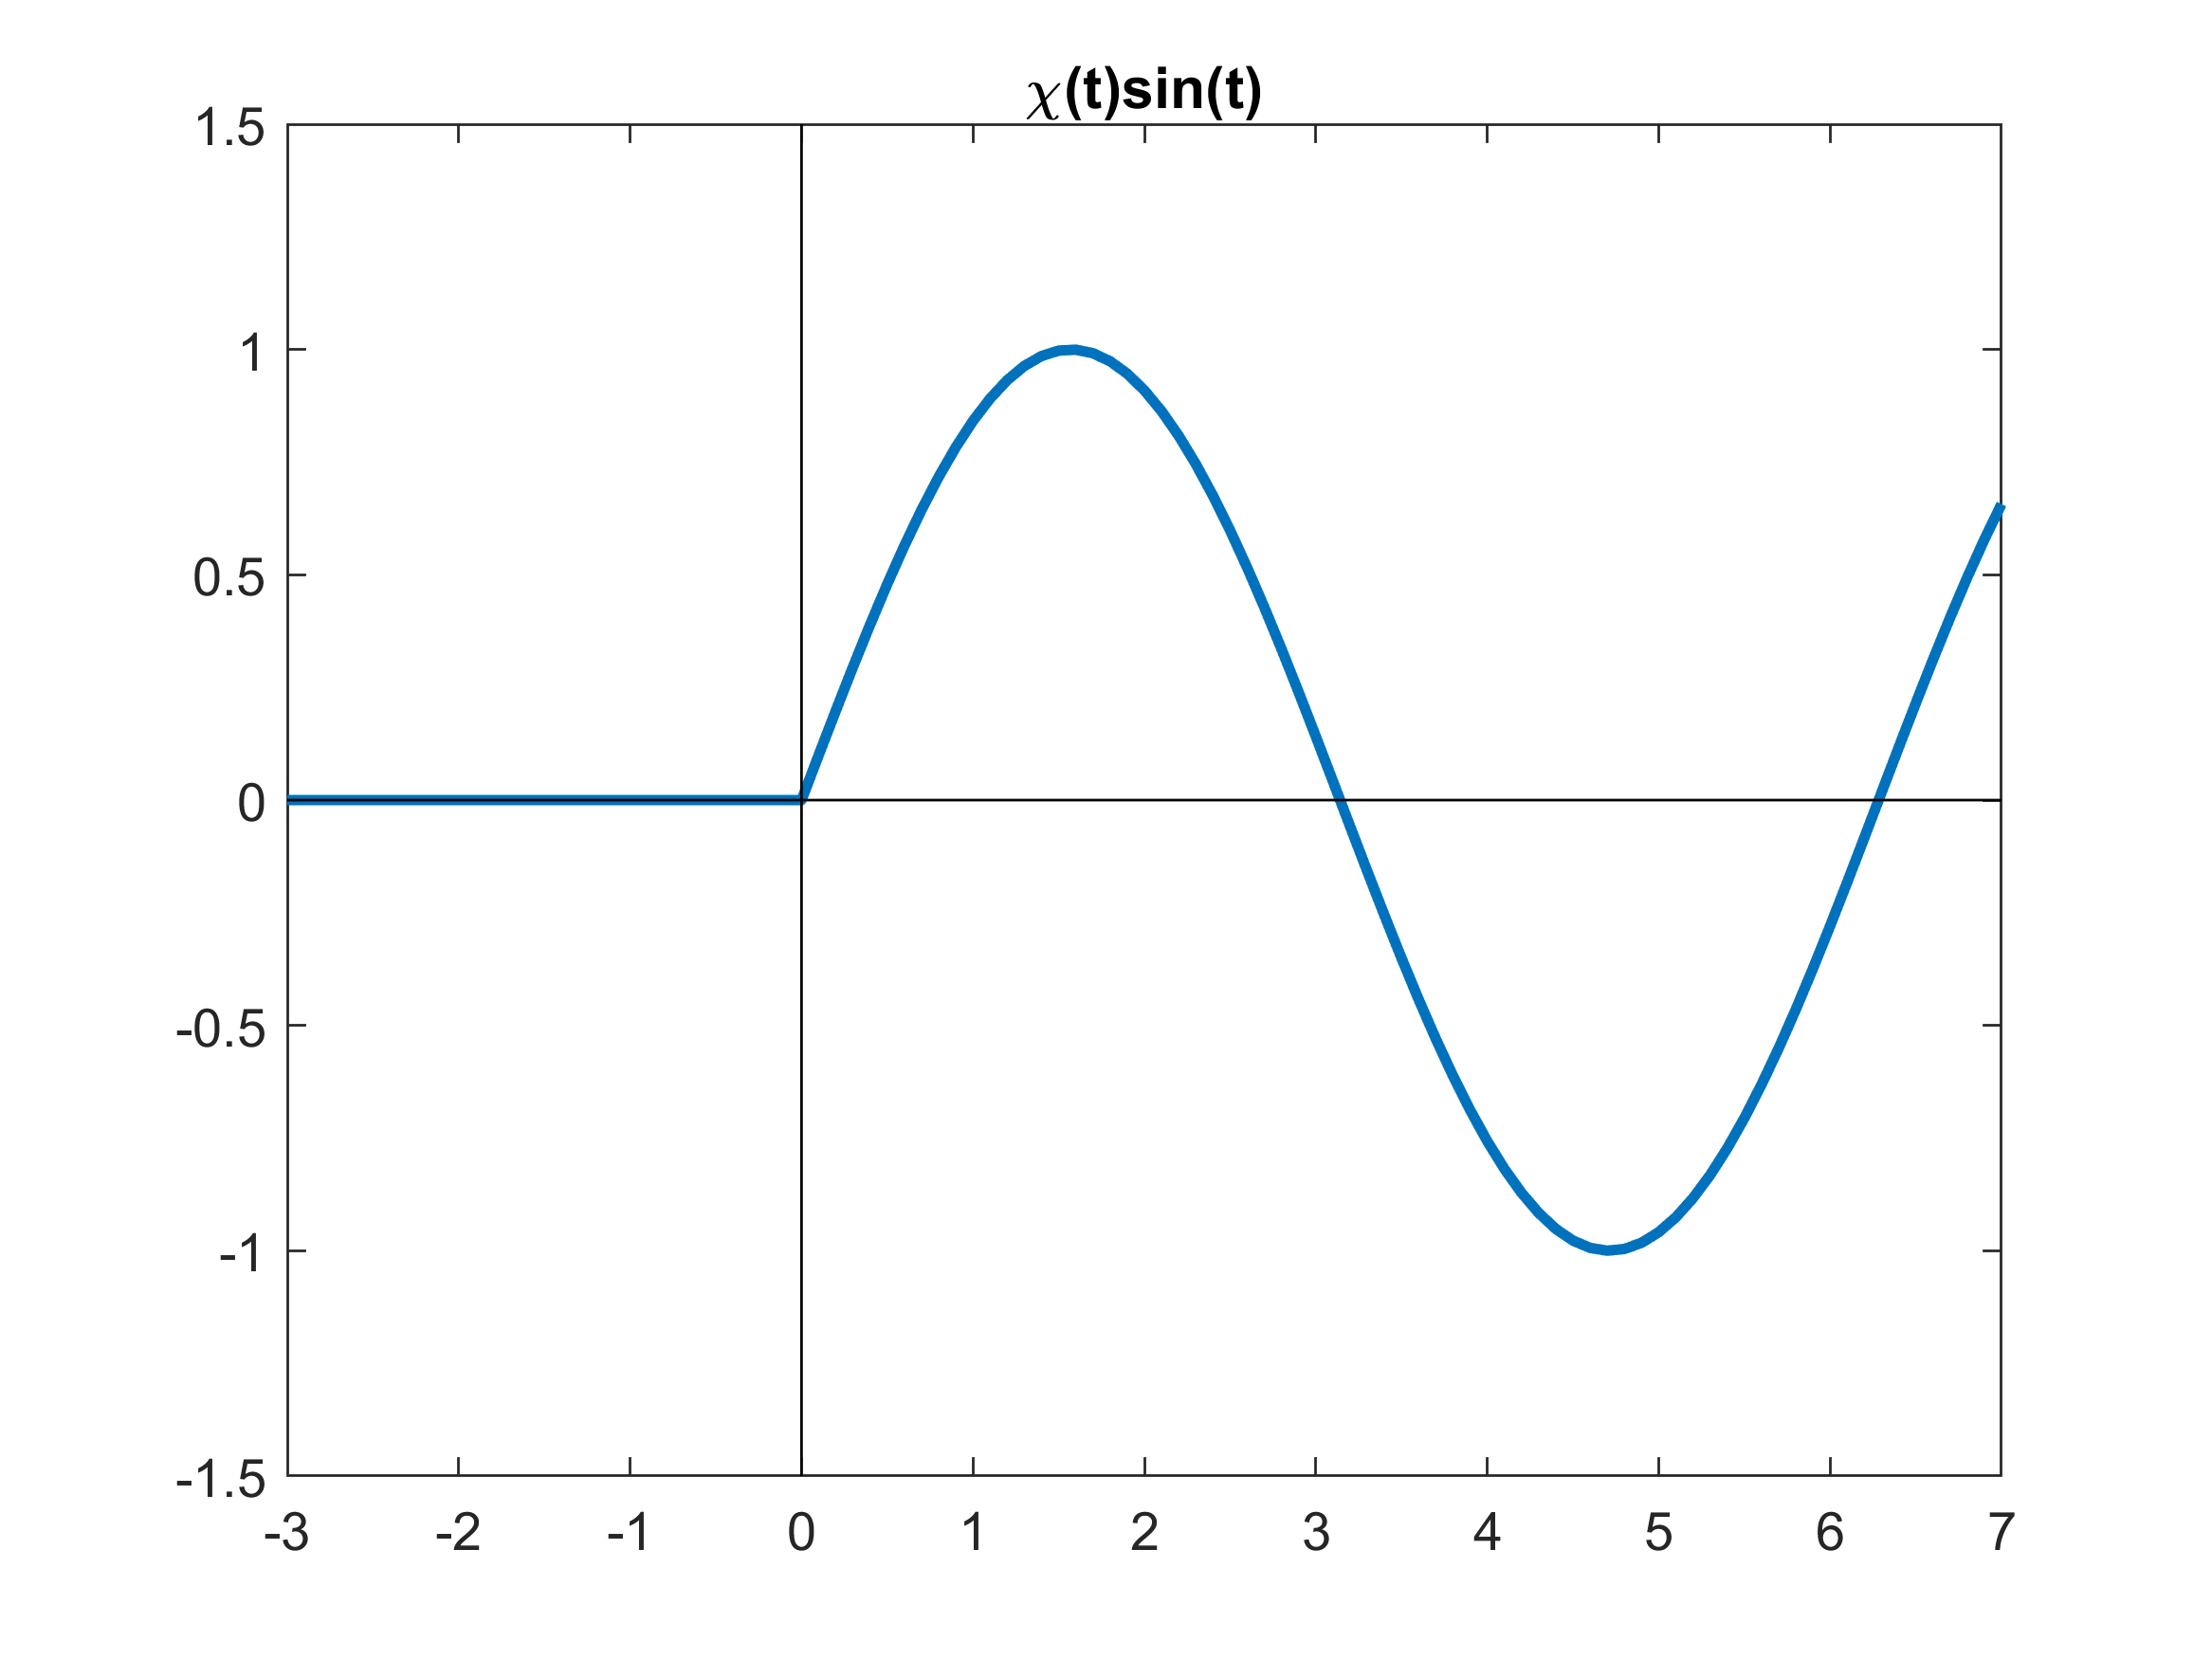
\includegraphics[width=0.9\textwidth]{pict/hev_pict.png}
			 			$$
			 				\chi(t)\sin(t) \lftKul \dfrac{1}{1+p^2}
						$$
			 		\end{minipage} \vspace{3mm}
			 			\hfill
					\begin{minipage}{0.45\textwidth}	
			 			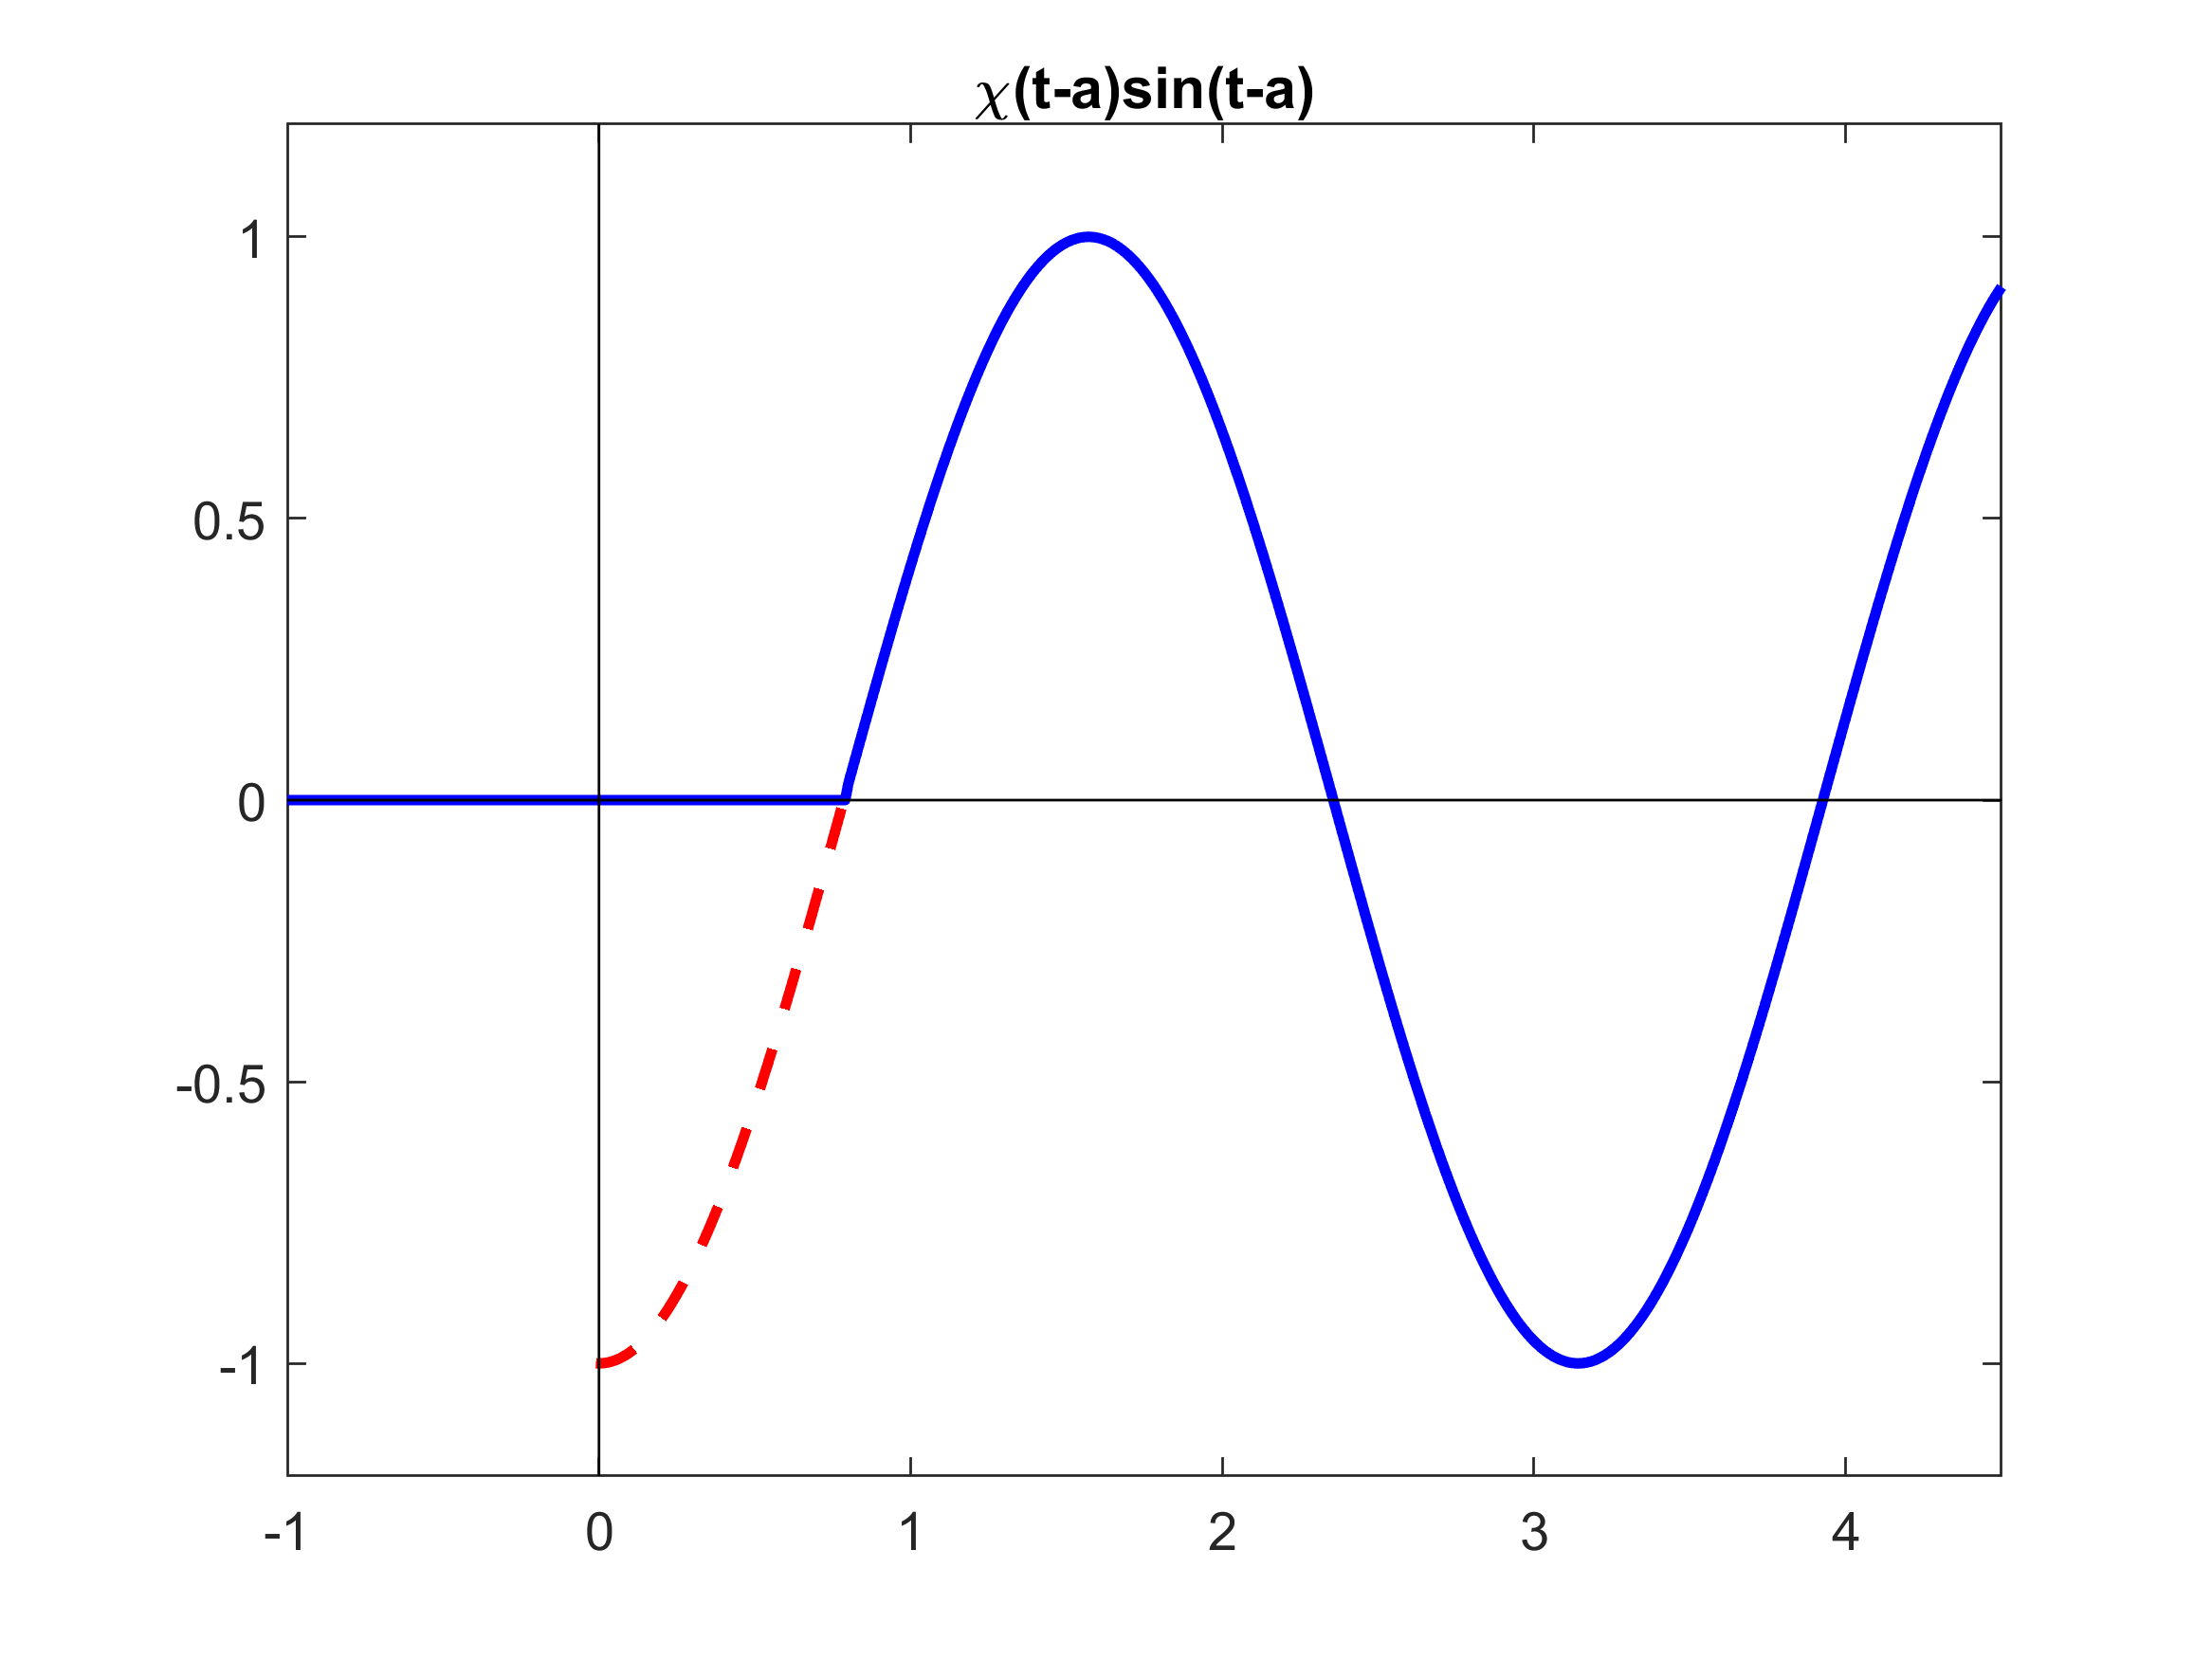
\includegraphics[width=0.9\textwidth]{pict/prop_1_2.png}
			 			$$
			 				\underline{\chi(t-1)}\sin(t-1) \lftKul \dfrac{e^{-p}}{1+p^2}
						$$
			 		\end{minipage} \vspace{3mm}
			 		$$
			 			\textbf{\large!} \quad 
			 				\underline{\chi(t)}\sin(t-1) \lftKul \dfrac{\cos(1)}{1+p^2} - \dfrac{\sin(1)p}{1+p^2}
			 			\quad \textbf{\large!} \qquad
			 			\left[ \quad \begin{gathered}
					 				\text{Мы знаем преобразования для $\chi(t)$,} \\
					 				\text{а у нас все с $a$ начинается здесь.} \\
					 				\text{Аккуратно с $\chi(t)$\textbf{!},}\\
					 				\text{нужно смотреть на аргумент.} 
					 				\,
					 			\end{gathered}  \quad
					 	\right] 
			 		$$ 
			 	\item 2-ая Th смещения \vspace{1mm} \newline
			 		$$
			 			\chi(t)f(t+a)  \lftKul e^{ap}\left[ F(p) - \int\limits_{0}^{+\infty} f(t) e^{-pt}dt \right],\,  a>0
			 		$$
			 		
			 		\begin{minipage}{0.45\textwidth}	
			 			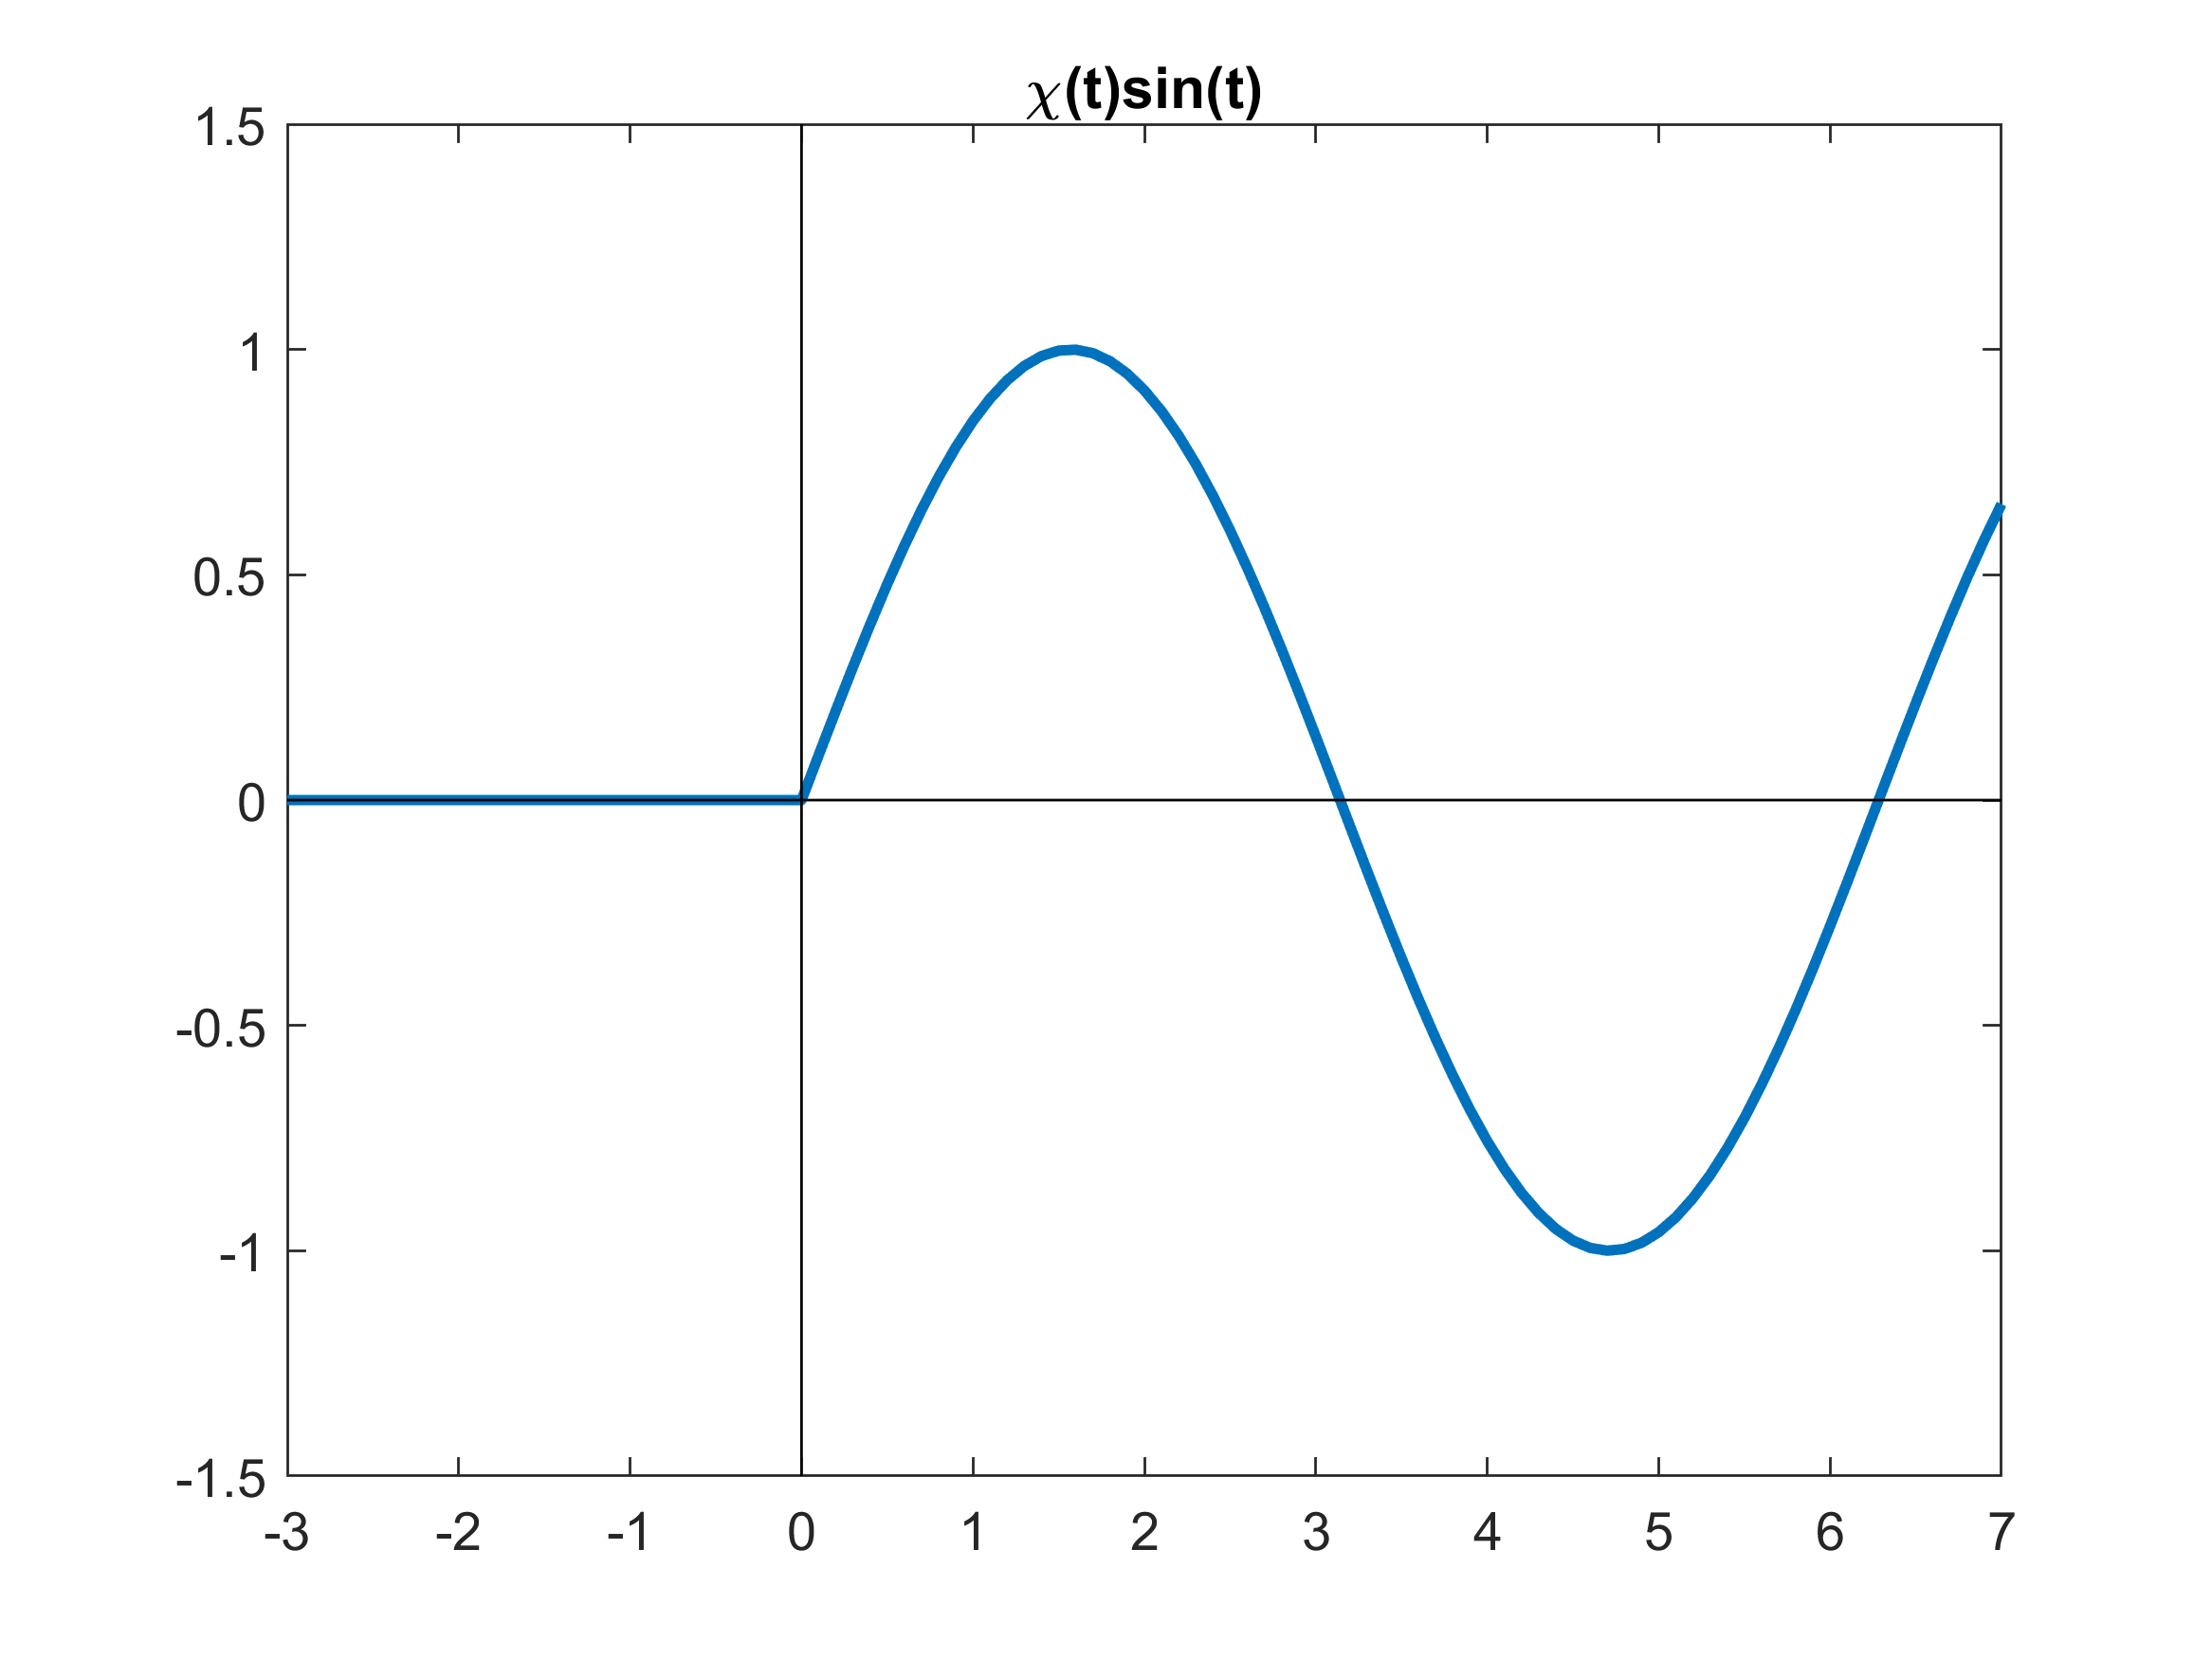
\includegraphics[width=0.9\textwidth]{pict/hev_pict.png}
			 		\end{minipage} \vspace{3mm}
			 			\hfill
					\begin{minipage}{0.45\textwidth}	
			 			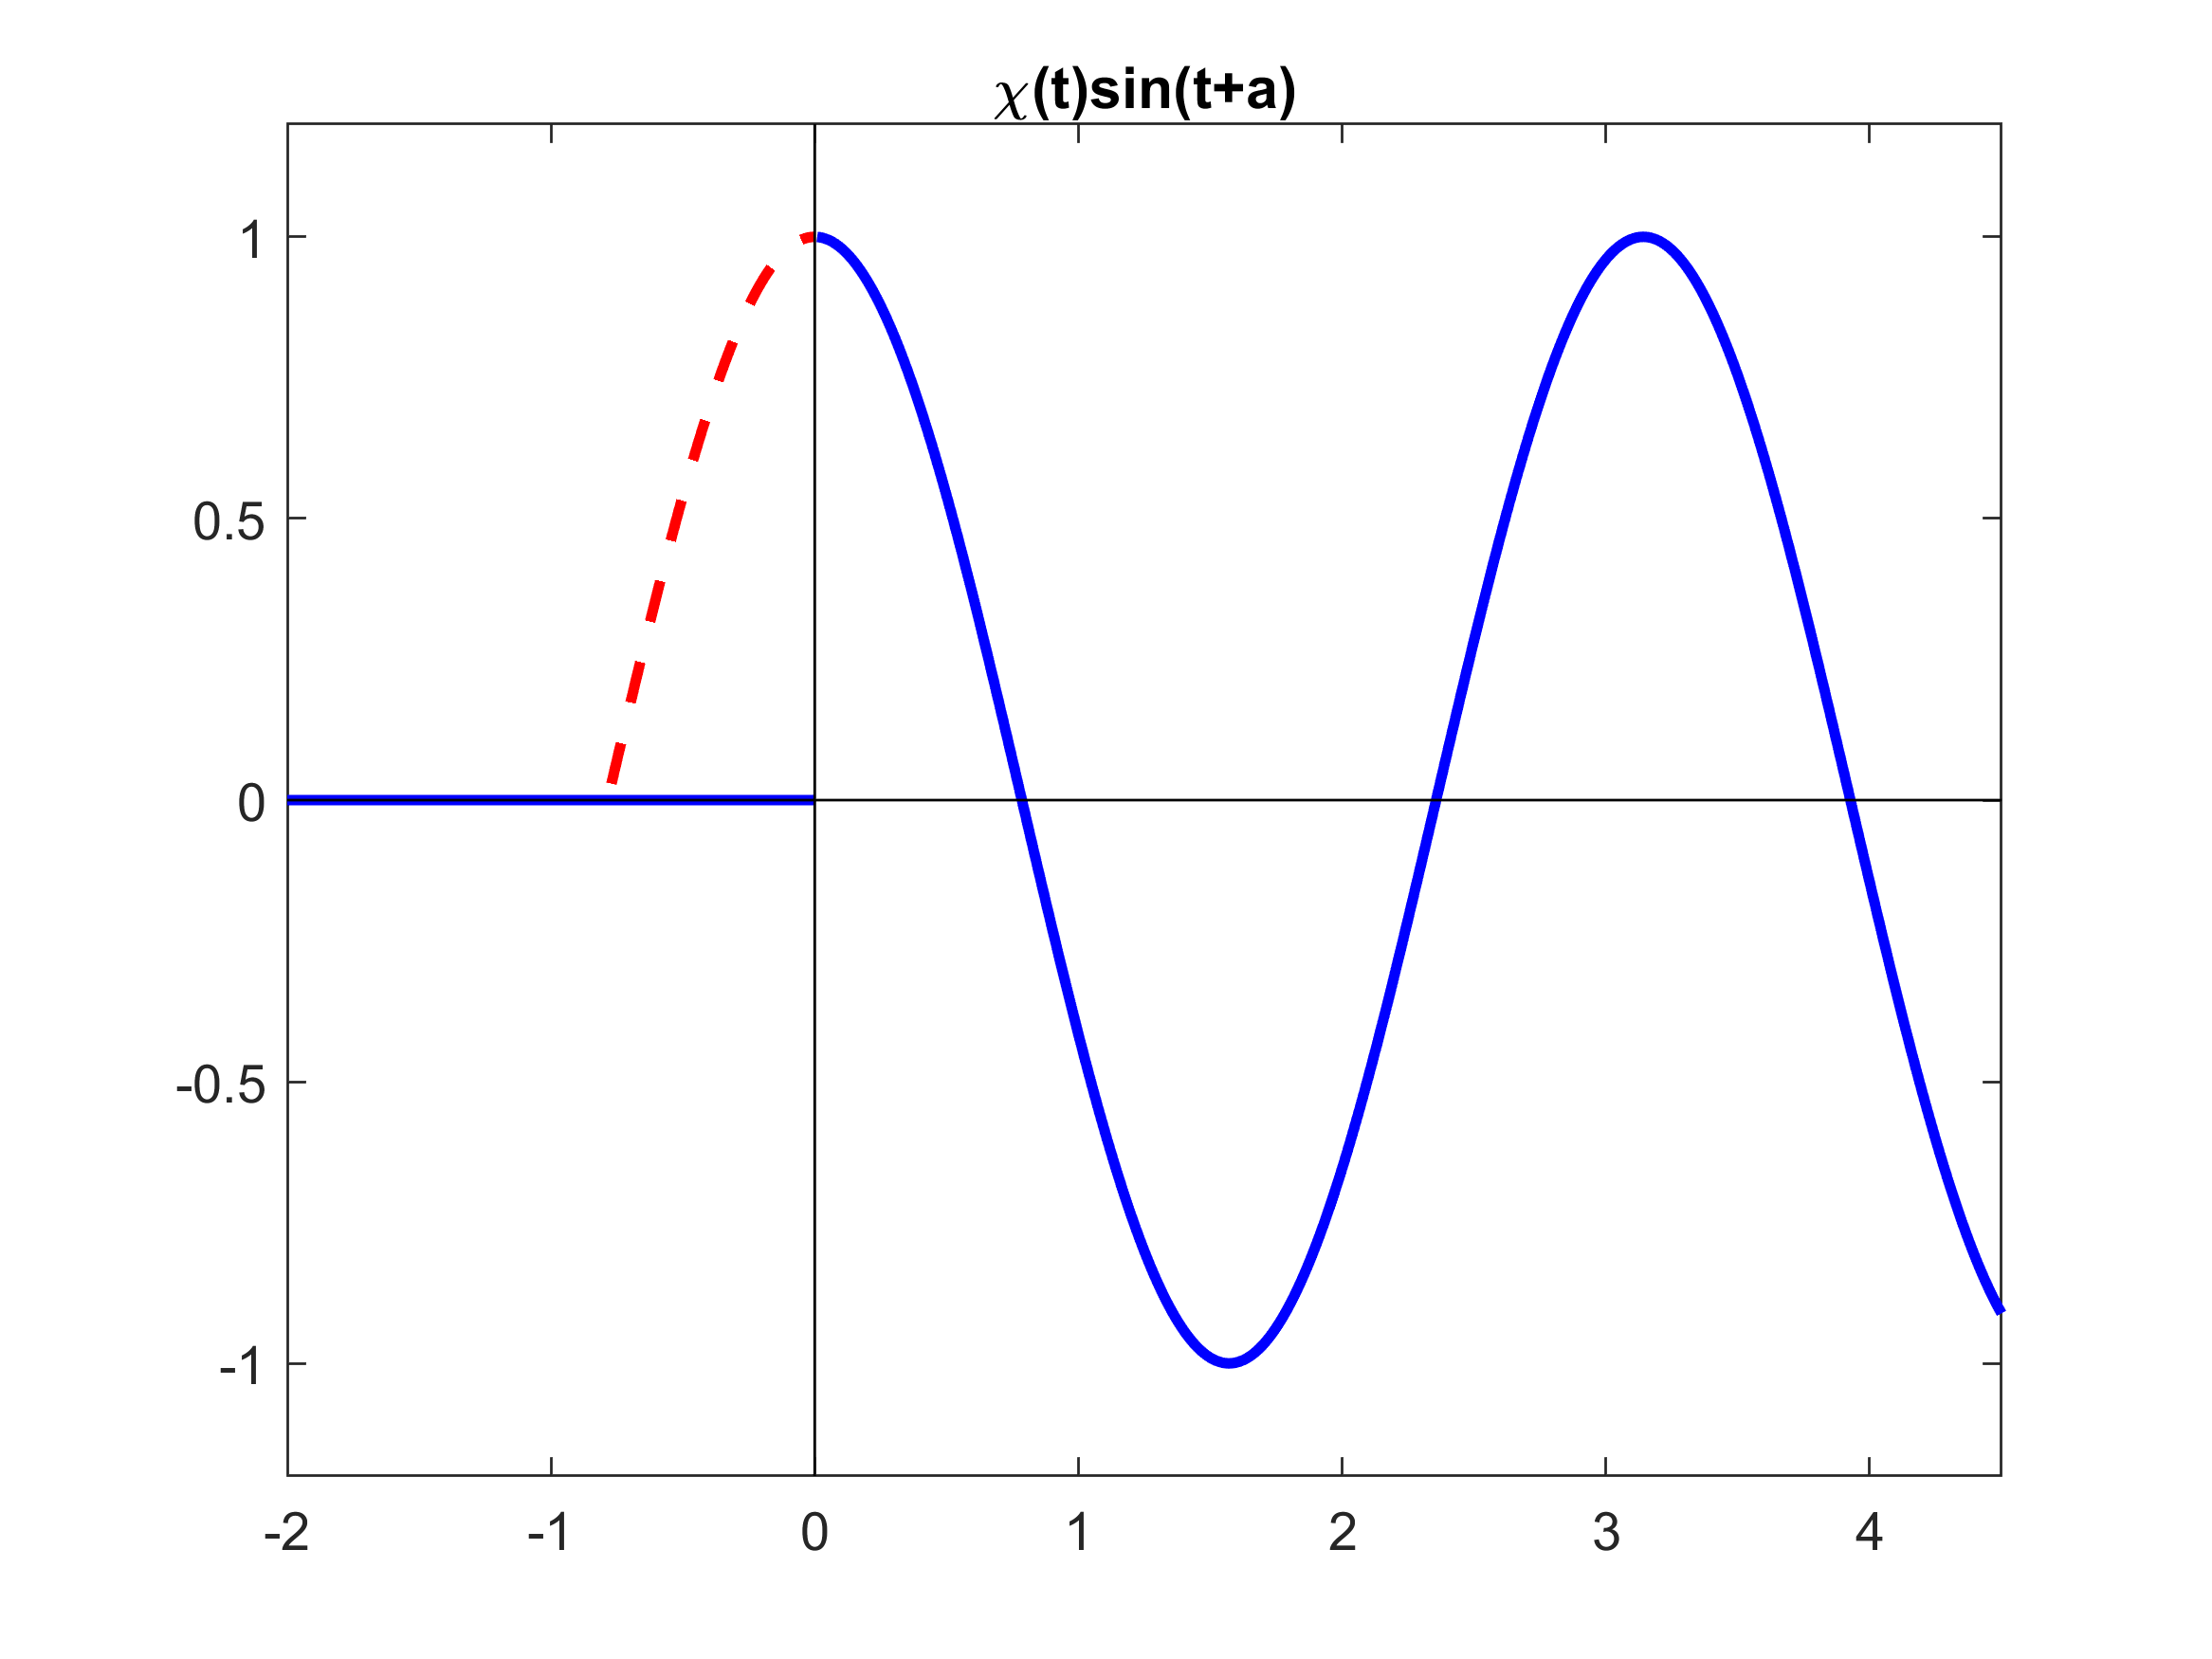
\includegraphics[width=0.9\textwidth]{pict/prop_2_2.png}
			 		\end{minipage} \vspace{3mm}
			 		$$
			 			 \int\limits_{0}^{+\infty} f(t+a) e^{-pt}dt = \{s=t+a\} 
			 			 = \int\limits_{a}^{+\infty} f(s) e^{-p(s-a)}dt
			 			 = e^{ap} \left[ F(p) - \int\limits_{0}^{a} f(t) e^{-pt}dt \right] 		
			 		$$ 
			 		\begin{center} Эта часть с минусом --- поправка на вылезшую за 0 часть графика. \end{center}
			 		\vspace{1mm}
			 	\item Th затухания  \newline
			 		$$
			 			\chi(t)f(t)e^{-\beta t} \lftKul F(p+\beta), \qquad \beta \in \mathbb{C}
			 		$$\vspace{1mm}
			 \end{enumerate}
		\item \textbf{Дифференцирование}
			\begin{enumerate}
			 	\item Дифференцирование оригинала
			 		$$ f \in \mathbb{C}^k(0,+\infty), \text{ т.е. } \exists f(+0), f'(+0), \cdots, f^{k-1}(+0)$$
			 		$$
			 			f^{(k)}(t) \lftKul p^k F(p) - p^0 f^{(k-1)}(+0) - p^1 f^{(k-2)}(+0) - \cdots - p^{k-1}f^{(0)}(+0) 
			 			\left| 	\begin{gathered}
			 							\text{ сумма степеней у частей} \\
			 							\text{ с минусом равна $k-1$ }
									\end{gathered}
						 \right.
			 		$$
			 		$$
			 			k=1: \qquad \int\limits_{0}^{\infty} f'(t) e^{-pt}dt  = f(t)e^{-pt}\Big|_{0}^{\infty} - 
			 										\int\limits_{0}^{\infty} (-p) f(t) e^{-pt}dt = pF(p) - f(+0)\vspace{2mm}
			 		$$
			 		
			 		\begin{itemize}
			 			\item Важность $f(+0)$ \vspace{3mm}\newline
			 				$\left. \chi(t) \lftKul \dfrac{1}{p} \qquad \qquad \right| \,\dfrac{d}{dt}\Big|_{t=0+}$
								\vspace{3mm} \newline
			 				$0 \lftKul 1 -\bsbKul1\,\leftarrow$ из $p^0f^{(k-1)}(+0)$ \quad Если $t=0$, то  $\nexists \chi'(0)$
											\vspace{3mm}  	
			 			\item Важность $\mathbb{C}^k(0,+\infty)$ \newline
			 				\begin{minipage}{0.3\textwidth}	
					 			$$
					 				\begin{gathered}
						 				\chi(t-1) \lftKul \dfrac{e^{-p}}{p} \quad  \Big| \dfrac{d}{dt}	\\
						 				0 \stackrel{?!}{\lftKul} e^{-p}\\
										\text{Противоречие т.к. } f(t) \not \in C^k(0;+\infty), \text{но} \vspace{3mm} \\
										\underline{\delta(t-1) \lftKul e^{-p}} \\
									\end{gathered}
								$$
								$$
										\int\limits_{0}^{\infty} \delta(t)  e^{-pt}dt \equiv 1 \qquad
										\int\limits_{0}^{\infty} \delta^{(k)}(t)  e^{-pt}dt \equiv p^{(k)}
								$$
					 		\end{minipage} \vspace{3mm}
					 			\hfill
							\begin{minipage}{0.45\textwidth}	\qquad
					 			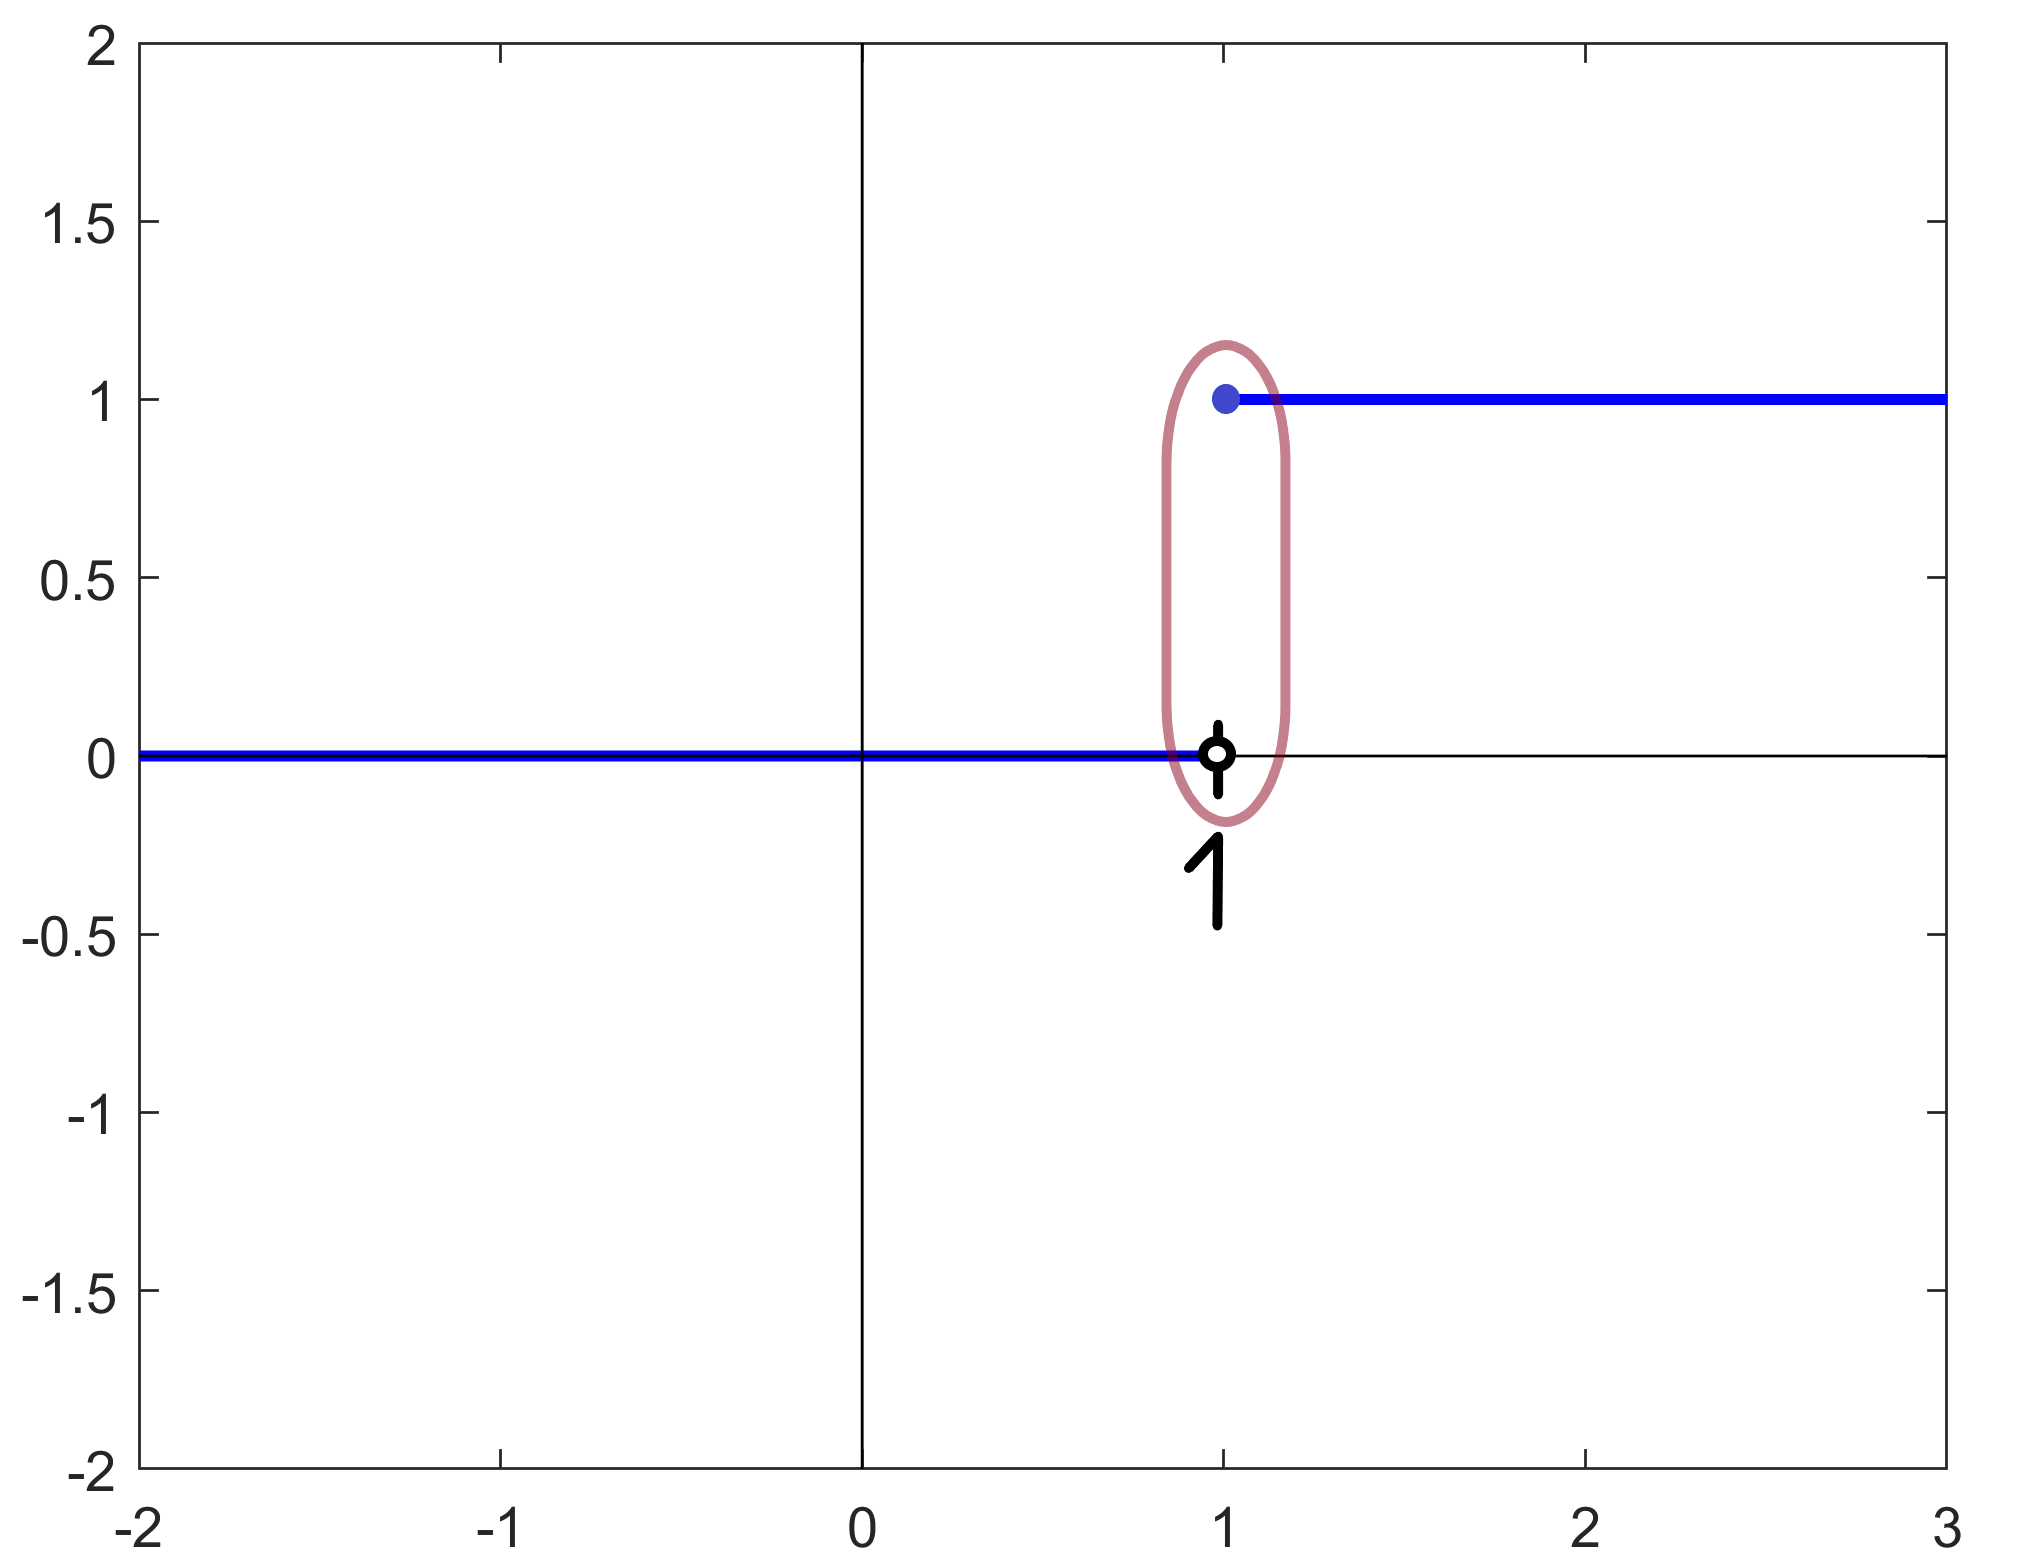
\includegraphics[width=0.9\textwidth]{pict/prop_3.png} \label{eq_1}
					 		\end{minipage} \vspace{3mm}
			 		\end{itemize}
			 	\item Дифференцирование изображения
			 		$$	\chi(t)(-t)^k f(t) \lftKul F^{(k)}(p) $$
			 \end{enumerate}
	\end{enumerate}
		
\end{document}
